\chapter{实验测试与分析}
\label{sec:Experiment}

在本章中,将给出基于真实世界数据集的评估结果,以证明本文针对加密重复数据删除提出的频率分析攻击方法的有效性(对加密重复数据删除的威胁的严重性)。

\section{实验方法}
\label{sec:dataset}

本文所使用的真实世界数据集不包数据的实际内容,因此基于数据块哈希模拟攻击者所拥有的的对抗性知识。具体来说,本文将一些快照中的有序的数据块哈希列表作为辅助信息$\mathbf{A}$和原始明文信息$\mathbf{M}$。为了模拟加密过程,在$\mathbf{M}$中的每个原始数据块哈希(表示明文)上应用额外的哈希函数,并将结果截断为当前使用的数据集中约定的哈希值的长度。截断的结果用于模仿$\mathbf{C}$中的密文。对于每个推理的密文数据块-明文数据块对$(C,M)$,本文通过在$M$上应用相同的模拟加密并将结果与​​$C$进行比较来验证其正确性。特别的,基于聚类的频率分析攻击可以在数据段级别进行操作,断出密文数据段-明文数据段对$(S_\mathbf{C},S_\mathbf {A})$。在这种情况下,本文通过检查$S_\mathbf{C}$中的每个密文是否完全映射到$S_\mathbf{A}$中的每个明文来评估$(S_\mathbf {C},S_\mathbf{A})$的正确性。

本文通过推理率和推理精度两个标准来衡量攻击的有效性(参见\ref{sec:ThreatModel})。


\section{基于分布的攻击的实验结果}
\label{sec:experiment-distribution}

\subsection{实验1(参数的影响)}
\label{sec:exp1}

本节将评估参数$(u, r, t)$的变化在基于分布的频率分析攻击中带来的影响。实验使用FSL数据集(参见\ref{sec:fsl})来进行评估。在实验中使用每个用户的第12周备份作为辅助信息来推理该用户相应的第14周备份中的原始明文数据。出于控制变量的需求,实验将在固定另两个参数的前提下对三个参数中的一个的变化进行测试和分析。


\subsubsection{参数$u$的影响}

首先,配置参数$t \rightarrow \infty$和$r = 0$来评估参数$u$变化的影响(在这种情况下,基于分发的攻击将退化到基于数据块局部性的的攻击\citing{li2017information})。

\begin{figure}[!htbp]
    \centering
    \begin{tabular}{p{.48\linewidth}p{.48\linewidth}}
        \multicolumn{2}{c}{
\includegraphics[width=.7\textwidth]{legend-fsl-line.pdf}}  \\
        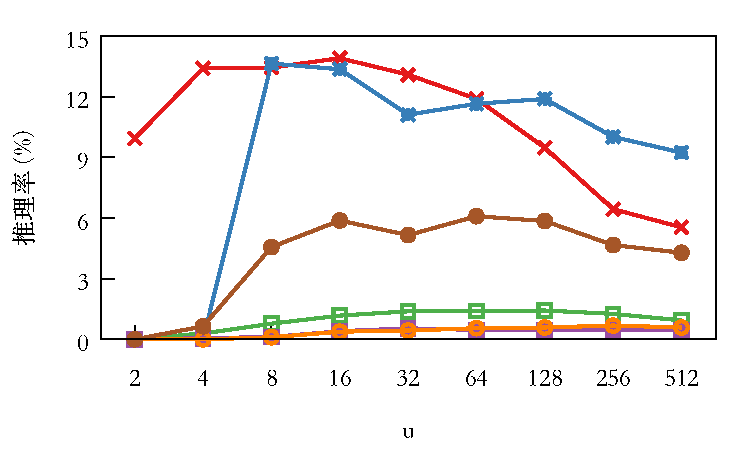
\includegraphics[width=\linewidth]{dis-impact-u-rate.pdf} &
        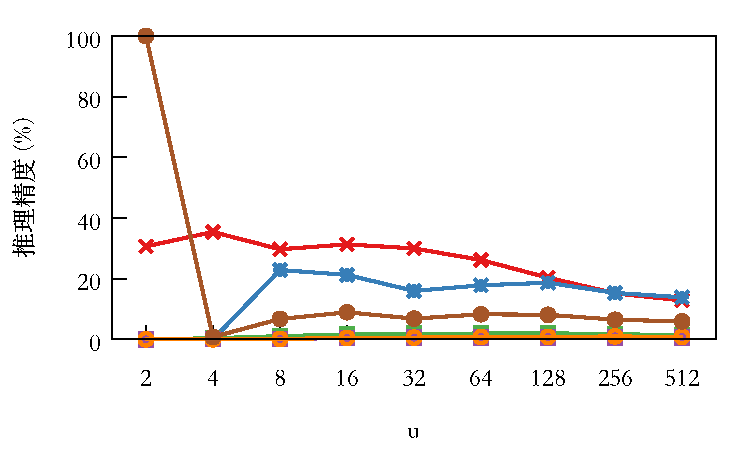
\includegraphics[width=\linewidth]{dis-impact-u-accuracy.pdf}\\
    \end{tabular}
    \caption{基于分布的攻击实验1:参数$u$的变化对推理结果的影响($r = 0$;$t \rightarrow \infty$)}
    \label{fig:distribution-impact-u}
\end{figure}

图\ref{fig:distribution-impact-u}显示了将参数$u$从2变为512时对推理率和推理精度带来的影响。对于推理率的结果,本实验的观察结果与已有的工作\citing{li2017information}相同。推理率首先随着$u$的增大而提高,这是因为频率分析攻击可以推理出更多的密文数据块-明文数据块对。推理率在达到最大值之后(例如,User004为13.9\%,User007为13.6\%,User012为1.4\%,User013为0.5\%,User015为0.7\%,User028为6.1\%)开始下降。其原因在于频率分析引入了大量的误报,这些误报会继续影响基于分布的攻击对每个数据块相邻邻居的推理。同时,部分特殊情况下的推理率约为0.0001\%,这意味着攻击只能推理出几个密文数据块-明文数据块对。

已有的工作\citing{li2017information}不提供基于数据块局部性的攻击的推理精度信息,因此本文提出的两种推理攻击方法的实验的推理精度的部分不与其进行对比。实验中观察到除User028的数据在$u=2$的条件下没有引入任何误报外,针对所有用户备份数据的推理精度都处于相当低的水平(小于40\%)。随着$u$的增大,推理精度会略有下降。例如,当$u$从2增加到512时,User004的推理精度从30.7\%下降到12.8\%。
    
\textbf{结论(1):}相对较大的$u$提高了推理率,但降低了推理精度(即,引入了更多的误报)


\subsubsection{参数$r$的影响}

然后,通过$u$变化的影响分析,本文选择增加推理的密文数据块-明文数据块对的覆盖范围,同时使用$r$和$t$来过滤可能的误报。因此,本文将User004,User013和User015的$u$设置为128,User007,User012和User028的设置分别为256,以评估$r$和$t$变化的影响。 

\begin{figure}[!htbp]
    \centering
    \begin{tabular}{p{.48\linewidth}p{.48\linewidth}}
        \multicolumn{2}{c}{
\includegraphics[width=.7\textwidth]{legend-fsl-line.pdf}}  \\
        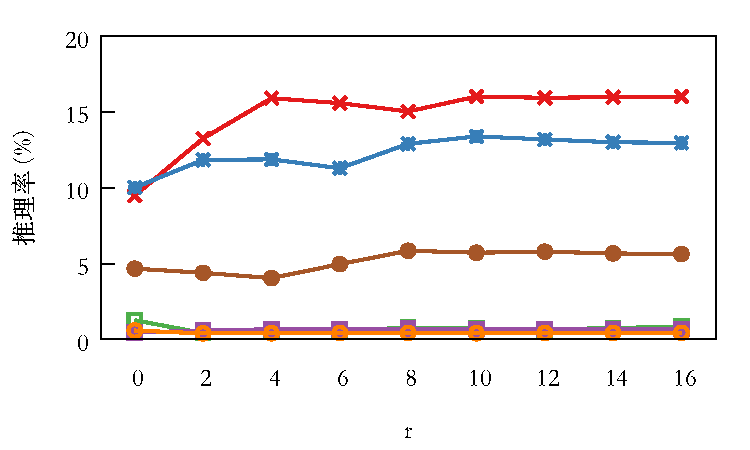
\includegraphics[width=\linewidth]{dis-impact-r-rate.pdf} &
        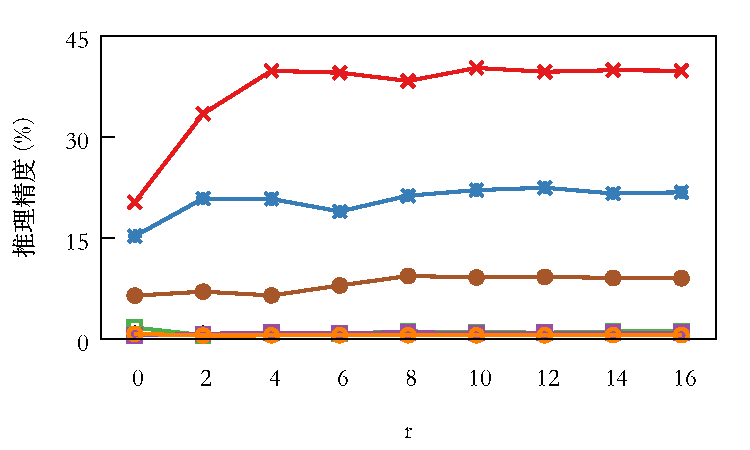
\includegraphics[width=\linewidth]{dis-impact-r-accuracy.pdf}\\
    \end{tabular}
    \caption{基于分布的攻击实验1:参数$r$的变化对推理结果的影响(User004、User013和User015中$u = 128$,User007、User012和User028中$u = 256$;$t \rightarrow \infty$)}
    \label{fig:distribution-impact-r}
\end{figure}

本实验中首先令$t\rightarrow \infty$,然后评估$r$变化带来的影响。图\ref{fig:distribution-impact-r}展示了参数$r$变化的实验结果。 实验观察到大多数用户的推理率随着$r$而增加。例如,当将$r$从0变为16时,User004推理率从9.5\%增加到16.0\%,User007从10.0\%增加到13.0\%,User013从0.5\%增加到0.7\%,User028从4.7\%增加到5.6\%。发生这种现象的原因是基于分布的攻击减少了直接频率排序的干扰,并推理出更多正确的密文数据块-明文数据块对。另一方面,对于User012和User015,推理率分别从1.3\%降至0.8\%,从0.6\%降至0.4\%。原因是随着检查的扩大,可能引入更多的误报。同时,所有用户的推理精度均处于低水平(小于45%),并且具有与其相应的推理率类似的变化趋势。


\textbf{结论(2):}较大的$r$提供了识别正确的密文数据块-明文数据块对的更多机会,但也增加了发生误报的概率。
\subsubsection{参数$t$的影响}

\begin{figure}[!ht]
    \centering
    \begin{tabular}{p{.48\linewidth}p{.48\linewidth}}
        \multicolumn{2}{c}{
\includegraphics[width=.7\textwidth]{legend-fsl-line.pdf}}  \\
        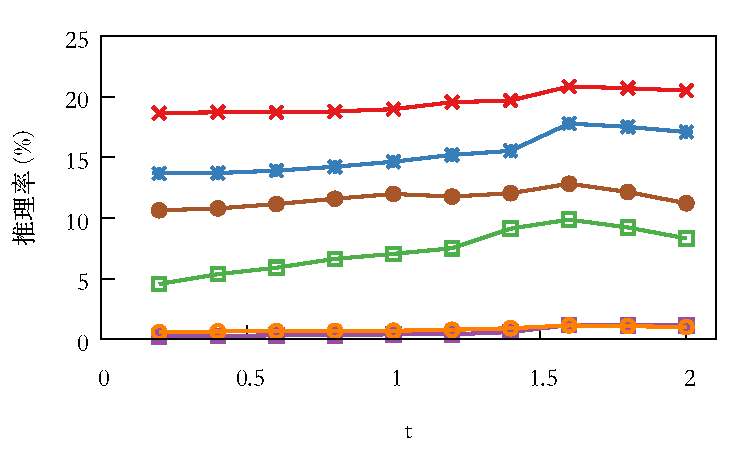
\includegraphics[width=\linewidth]{dis-impact-t-rate.pdf} &
        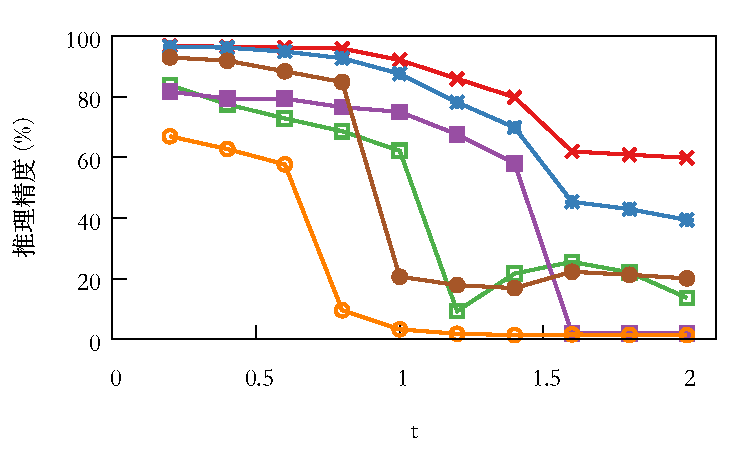
\includegraphics[width=\linewidth]{dis-impact-t-accuracy.pdf}\\
    \end{tabular}
    \caption{基于分布的攻击实验1:参数$t$的变化对推理结果的影响(User004、User013和User015中$u = 128$,User007、User012和User028中$u = 256$;$r = 10$)}
    \label{fig:distribution-impact-t}
\end{figure}

最后,设定$r=10$来评估参数$t$变化的影响。 图\ref{fig:distribution-impact-t}展示了参数$t$变化的实验结果果。当$t$很小(例如,小于0.5)时,实验观察到攻击误判并过滤了大量的密文数据块-明文数据块对,即使它们是正确的(即,引入了降低推理率的假阳性结果)。随着$t$的增加,假阳性的结果数量减少。当$t= 1.5$时,对于User004,User007,User012,User013,User015和User028,推理率分别达到最大值21.2\%,18.2\%,10.4\%,1.2\%,1.2\%和13.5\%。 当$t$进一步增大到2时,相应的推理率分别降至20.5\%,17.1\%,8.3\%,1.2\%,1.0\%和11.2\%。其原因是如果$t$过大,攻击就无法有效地过滤误报。因此,所有用户数据的推理精度都会随着$t$的增大而下降。

\textbf{结论(3):}较小的$t$过滤了大部分频率分析带来的误报,但它引入了更多的假阳性结果,导致了推理率的下降。

\subsection{实验2(与已有工作的对比)}
\label{sec:exp2}
本文将基于分布的攻击的有效性与基于数据块局部性的攻击的有效性进行比较\citing{li2017information}。除了使用实验1(参见\ref{sec:exp1})中采用的FSL数据集之外,本文还加入MS数据集(参见\ref{sec:ubc-ms})用于进行跨数据集的验证与评估。在MS数据集中,对于每个系统类别,一次选择两个快照,使用其中一个来推理另一个,以此评估平均的推理率和推理精度。

本文考虑采用以下攻击实例来进行比较。

\begin{itemize}[leftmargin=*]
\item \textbf{$\tt Baseline$:}

实验根据已有工作\citing{li2017information}中建议的参数配置实现基于数据块局部性的攻击。具体来说,它在频率分析的第一次调用中推理出5个出现频率最高的的密文数据块-明文数据块对(即,初始化一组用于迭代的密文数据块-明文数据块对),并且在每次后续调用中根据已有数据块对的邻居推理30个新的数据块对(即,迭代地推理密文数据块-明文数据块对)。

\item \textbf{$\tt Distribution$和$\tt Distribution^S$:} 

考虑两个基于分布的攻击的攻击实例,分别由$\tt Distribution$和$\tt Distribution^S$表示,它们分别使用和不使用大小信息作为辅助信息(即上标$\tt S$表示攻击实例使用大小信息进行操作)。实验在与${\tt Baseline}$相同参数的条件下配置$\tt Distribution^S$和${\tt Distribution}$。 此外,实验通过以下方式在$\tt Distribution^S$和${\tt Distribution}$中选择参数$r$和$t$的取值:对于FSL数据集,我们为所有用户设定$r = 10$,并分别为User004、User007、User012、User013、User015和User028设置参数$t$ = 1.5、1.2、1、1、0.7和0.9;对于MS数据集,实验继续为所有类别设置参数$r = 10$,为Win7和Serv-08设置参数$t = 2$,为Vista-U、Serv-03和Vista-B设置参数$t = 1.6$。以上数据是通过按照实验1(参见\ref{sec:exp1})的方法对数据集的最佳配置的测试得出的。 
\item \textbf{$\tt Distribution$-$\tt o$和$\tt Distribution^S$-$\tt o$:}

实验考虑另外两个基于分布的攻击的实例,用$\tt Distribution$-$\tt o$和$\tt Distribution^S$-$\tt o$表示,对于$r$和$t$应用与$\tt Distribution$和$\tt Distribution^S$相同的配置,但进一步使用更大的参数$u$增加推理的密文数据块-明文数据块对的覆盖范围。具体来说,实验通过以下方式在$\tt Distribution$-$\tt o$和$\tt Distribution^S$-$\tt o$中配置参数$u$:对于FSL数据集,参数$u$的选择与实验1(参见\ref{sec:exp1})相同;对于MS数据集,实验为Win7数据设置$u = 128$,为Serv-03、Serv-08、Vista-B和Vista-U设置$u  = 30$。 
\end{itemize}

\begin{figure*}[!htbp]
    \centering
    \begin{tabular}{c}
        
\includegraphics[width=.7\textwidth]{pic/legend-fsl-bar.pdf}\\
        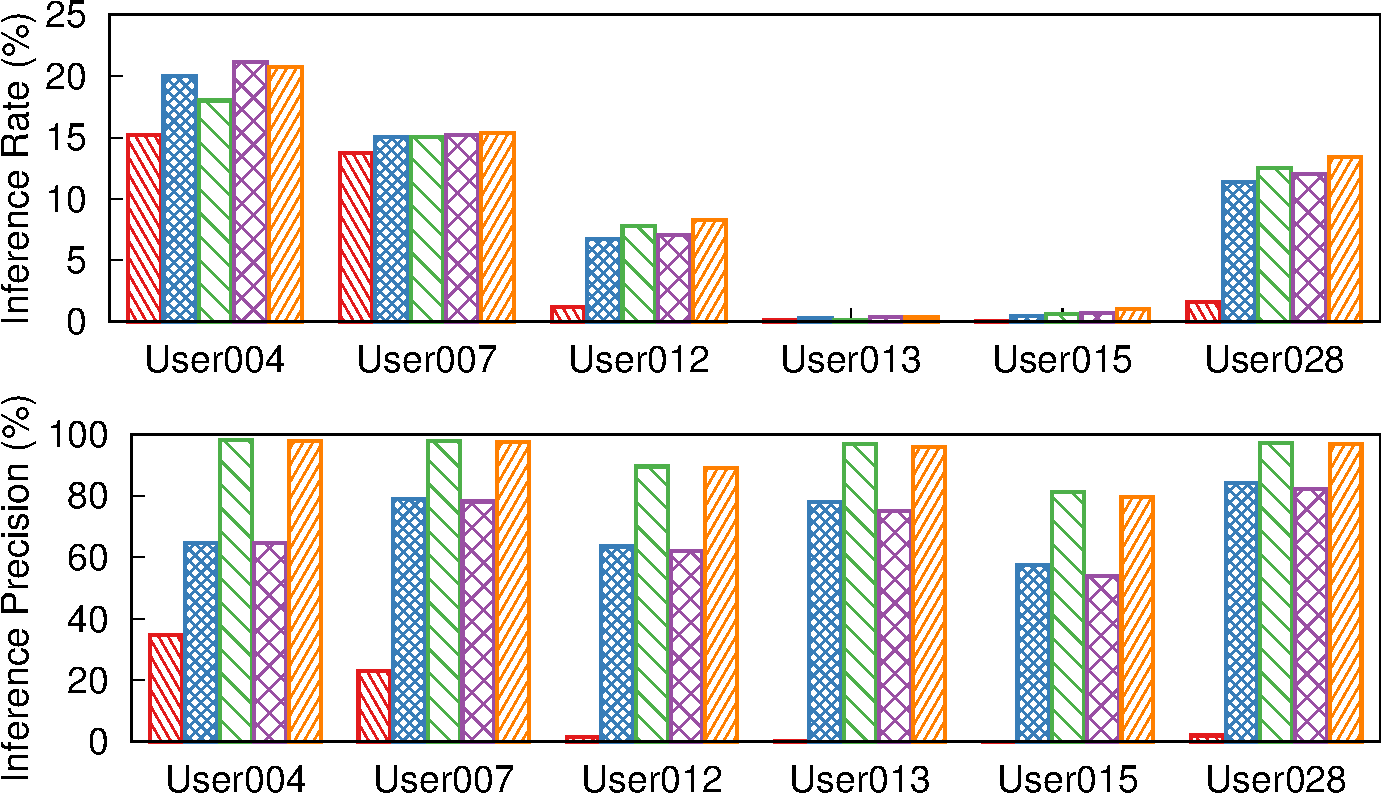
\includegraphics[width=.7\textwidth]{pic/distribution-comparison-fsl.pdf} 
    \end{tabular}
    \caption{基于分布的攻击实验2(与已有工作的对比):比较基于分布的攻击和基于数据块局部性的攻击的有效性(FSL数据集)。}
    \label{fig:distribution-comparison-fsl}
\end{figure*}

图\ref{fig:distribution-comparison-fsl}给出了基于FSL数据集的上述5种实例的比较结果。实验观察到,在几乎所有情况下,基于分布的攻击的不同实例都优于基于数据块局部性的攻击。例如,对于User028,基于分布的攻击的最低推理率是11.4\%,推理精度为84.1\%($\tt Distribution$);此时$\tt Baseline$相应的推理率仅为1.2\%,推理精度仅为1.7\%。这意味着在这种情况下,基于分布的攻击可以将假阳性的数量减少82.4\%。

\textbf{结论(4):}基于分布的攻击显着提高了推理精度,同时实现了比基于数据块局部性的攻击更高的推理率。 

$\tt Distribution^S$和$\tt Distribution^S$-$\tt o$相较于$\tt Distribution$和$\tt Distribution$-$\tt o$拥有更高的推理精度,这因为它们进一步通过数据块大小信息过滤了误报。例如,对于User004,$\tt Distribution^S$和$\tt Distribution^S$-$\tt o$相较于$\tt Distribution$和$\tt Distribution$-$\tt o$将误报分别从35.2\%减少到1.7\%,从35.3\%减少到2.2\%。然而,在同样的情况下,实验观察到$\tt Distribution$ and $\tt Distribution$-$\tt o$的推理率分别为20.0\%和21.2\%,相较于$\tt Distribution^S$和$\tt Distribution^S$-$\tt o$分别高出2.0\%和0.4\%。其原因是$\tt Distribution$和$\tt Distribution$-$\tt o$推理出了来自不正确的密文数据块-明文数据块对的邻居中的少量正确结果。换句话说,虽然$(C, M)$是不正确的密文数据块-明文数据块对,但$C$的邻居可能以很小的概率对应于$M$的邻居。即使在这种情况下,所有基于分布的攻击实例都比基于数据块局部性的攻击实例效果更佳。具体来说,$\tt Baseline$的推理率仅为15.2\%,比基于分布的攻击的最佳情况低6.0\%,最差情况低2.8\%。  

\textbf{结论(5):}过滤不正确的推理结果可以提高推理精度,但会降低推理的密文数据块-明文数据块对的覆盖范围,并可能降低推理率。

我们进一步观察到,虽然$\tt Distribution$-$\tt o$和$\tt Distribution^S$-$\tt o$构建在更大的参数$u$上,但它们的推理率仅略高于$\tt Distribution$和$\tt Distribution^S$(分别高为0.4\%和0.9\%)。 原因是基于分布的攻击仅通过已推理出数据块对的邻居进行迭代推理。参数$u$的进一步增大只会在结果中添加少量新的正确密文数据块-明文数据块对。

\begin{figure*}[t]
    \centering
    \begin{tabular}{c}
        
\includegraphics[width=.7\textwidth]{pic/legend-fsl-bar.pdf}\\
        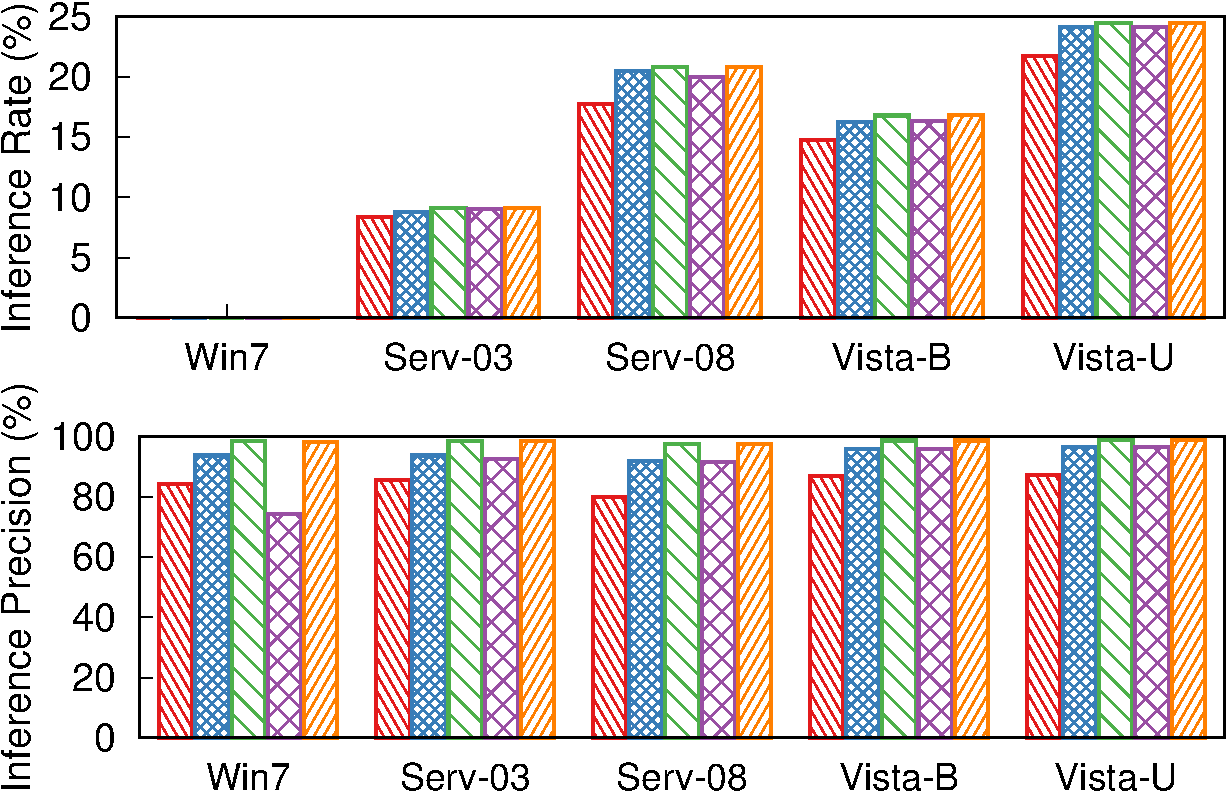
\includegraphics[width=.7\textwidth]{pic/distribution-comparison-ms.pdf}\\
    \end{tabular}
    \caption{基于分布的攻击实验2(与已有工作的对比):比较基于分布的攻击和基于数据块局部性的攻击的有效性(MS数据集)。}
    \label{fig:distribution-comparison-ms}
\end{figure*}


图\ref{fig:distribution-comparison-ms}给出了基于MS数据集的上述5种实例的比较结果。基于数据块局部性的攻击和基于分布的攻击在大多数MS数据集的类别(Win7除外)中具有高推理率和精度。可能的原因是MS数据集中的快照高度相关(例如,数据块总数的方差很小,如表\ref{tab:MS-dataset}所示)。实验观察到基于分布的攻击仍然优于基于数据块局部性的攻击。例如,在Vista-U中,基于分布的攻击的所有推理的推理率和推理精度分别高于24.1\%和96.4\%,而$\tt Baseline$的推理率和分辨率分别为21.7\%和87.1\%。

实验中对于数据集中Win7类别,基于分布的攻击和基于数据块局部性的攻击的推理率都很低(小于0.01%)。其原因是Win7包含大量具有唯一性的数据块(大约超过98.8\%,如表\ref{tab:MS-dataset}所示),导致了攻击效果表现不佳。

\subsection{实验3(攻击效果)} 
\label{sec:exp3}
实验考虑长期备份模式,并使用FSL数据集检查基于分布的攻击的有效性。具体来说,实验选择每个用户的第$i$个FSL每周备份作为辅助信息,以推理相应的第$(i+w)$个FSL每周备份中的原始明文。显然,$w$越小,辅助信息和目标备份之间的相关性就越高。与实验2(参见\ref{sec:exp2})配置两个基于分布的攻击实例$\tt Distribution$-$\tt o$和$\tt Distribution^S$-$\tt o$,并评估它们的推理率和推理精度(针对每个用户的所有可用的$i$)。

\begin{figure*}[!htbp]
    \centering
    \centering
    \begin{tabular}{c}
        
\includegraphics[width=.35\textwidth]{legend-effectiveness.pdf}\\
        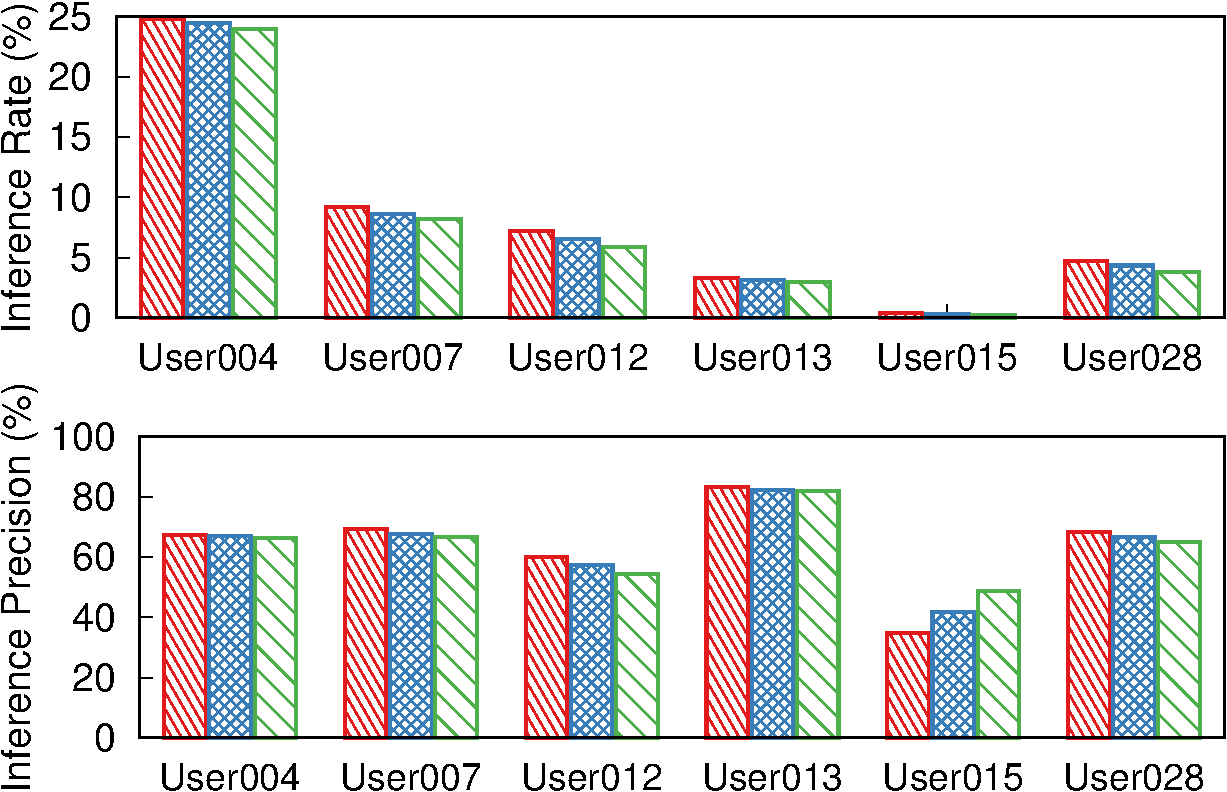
\includegraphics[width=.7\textwidth]{distribution-effectiveness-wo-size.pdf}
    \end{tabular}
	\caption{实验3(攻击效果):没有大小信息辅助的基于分布的攻击在FSL数据集中的有效性。}
	\label{fig:experiment-distribution-effectiveness-wo}
\end{figure*}

图\ref{fig:experiment-distribution-effectiveness-wo}给出了$\tt Distribution$-$\tt o$的实验结果。基于分布的攻击在用户之间具有不同的推理率和推理精度。例如,在类似User004这样的有利情况下,它实现了推理率24.8\%、推理精度67.3\%($w = 1$);推理率24.5\%、推理精度67.0\%($w = 2$);推理率24.0\%、推理精度66.5\%($w = 3$)。在类似User015这样的非有利情况下,基于分布的攻击的推理率仅有0.3\%。可能的原因是User015的备份数据具有较低的数据块局部性。

此外,实验观察到辅助信息的相关性(即$w$)对基于分布的攻击的有效性影响较低。例如,当$w$从1增加到3时,它仅导致推理率(下降小于1.4\%)和精度(下降小于5.6\%)的有限下降。其原因是基于分布的攻击解决了频率排名中的干扰并保留了攻击的有效性。

\textbf{结论(6):}基于分布的攻击可以在存在松散相关的辅助信息的帮助下有效控制攻击有效性的下降程度。

\begin{figure*}[!htbp]
    \centering
    \centering
    \begin{tabular}{c}
        
\includegraphics[width=.35\textwidth]{pic/legend-effectiveness.pdf}\\
        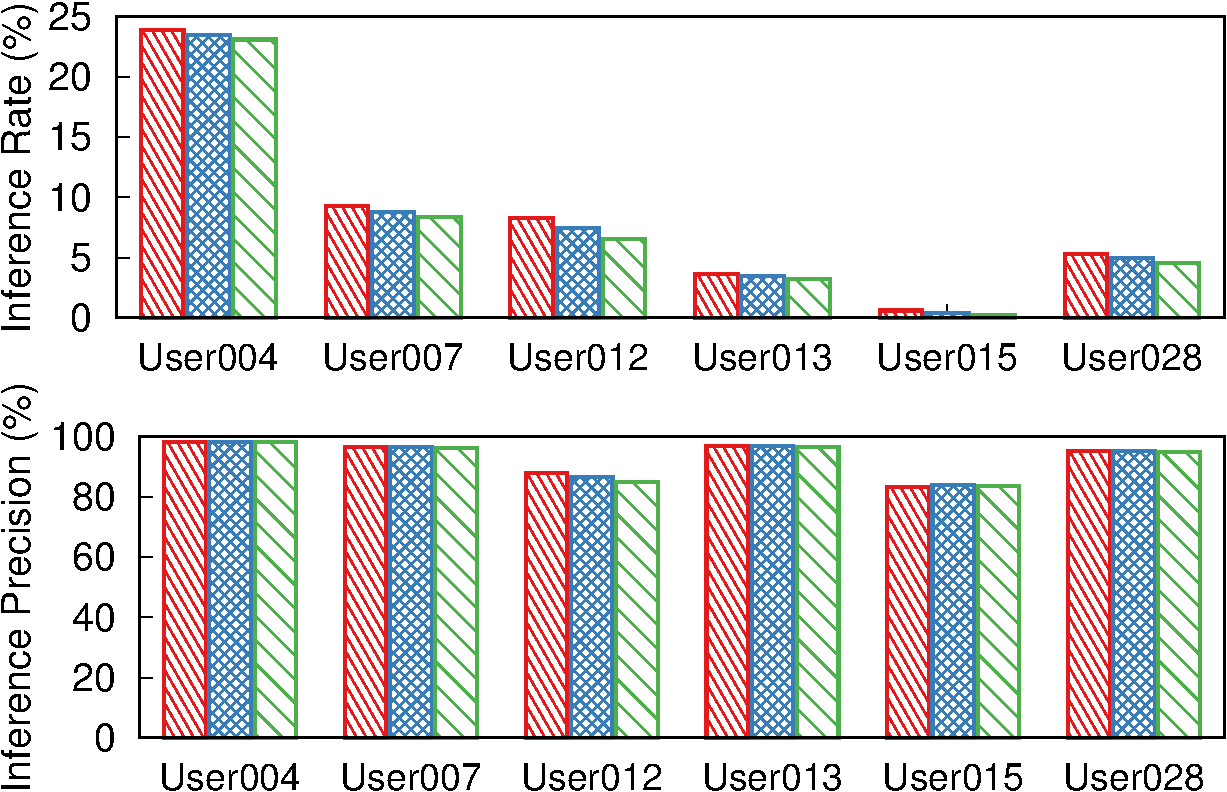
\includegraphics[width=.7\textwidth]{pic/distribution-effectiveness-w-size.pdf}
    \end{tabular}
	\caption{实验3(攻击效果):有大小信息辅助的基于分布的攻击在FSL数据集中的有效性。}
	\label{fig:experiment-distribution-effectiveness-w}
\end{figure*}

图\ref{fig:experiment-distribution-effectiveness-w}给出了$\tt Distribution^S$-$\tt o$的实验结果。实验观察到它具有与$\tt Distribution$-$\tt o$相似的推理率,同时拥有更高的推理精度。例如,对于所有用户的平均推理精度分别为93.1\%($w = 1$)、92.8\%($w = 2$)和92.4\%($w = 3$)。         

\section{基于聚类的攻击的实验结果}
\label{sec:experiment-clustering}

\subsection{实验4(参数的影响)} 
\label{sec:exp4}
实验首先评估参数$k$的影响,该参数定义了凝聚法层次聚类中组合两个最近聚类的距离上限。本实验使用FSL和VM数据集来研究$k$如何影响攻击中的基础聚类方案。具体来说,分别对每个选出的FSL和VM用户数据的最后一次备份应用分段方法,并生成固定大小为4MB的数据段。

聚类方案旨在将类似的密文数据段聚合到同一个聚类中,这一过程不会损害每个密文数据段中的数据块的机密性。本文使用聚类接近度量化其影响,将聚类的结果与实际分类方法的结果进行比较(实际分类方法通过最小数据块哈希直接对分段进行分类)。假设我们分别通过实际分类方法生成$m$个数据段的集合,并且通过聚类方案生成$\widetilde{m}$个数据段的集合。通过$\frac{{\sf abs}(m-\widetilde{m})}{m}$(其中${\sf abs}(m-\widetilde{m})$返回$m-\widetilde{m}$的绝对值)衡量聚类形成的集合与实际分类形成的集合的相似程度。记集合所有数据段都相同(具有相同的最小数据块哈希)的聚类的数量为$\hat{m}$。此外,实验还考虑了聚类正确性,通过$\frac{\hat{m}}{\widetilde{m}}$进行评估,它量化了对相似数据段的聚类方案的精确程度。

\begin{figure}[!htbp]
    \centering
    \begin{tabular}{p{.48\linewidth}p{.48\linewidth}}
        \multicolumn{2}{c}{
\includegraphics[width=.5\textwidth]{clu-fsl-bar.pdf}}  \\
        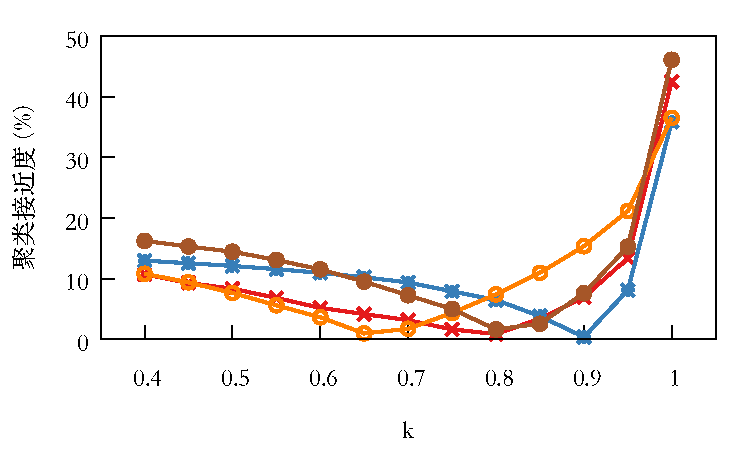
\includegraphics[width=\linewidth]{clu-impact-d-fsl-clo.pdf} &
        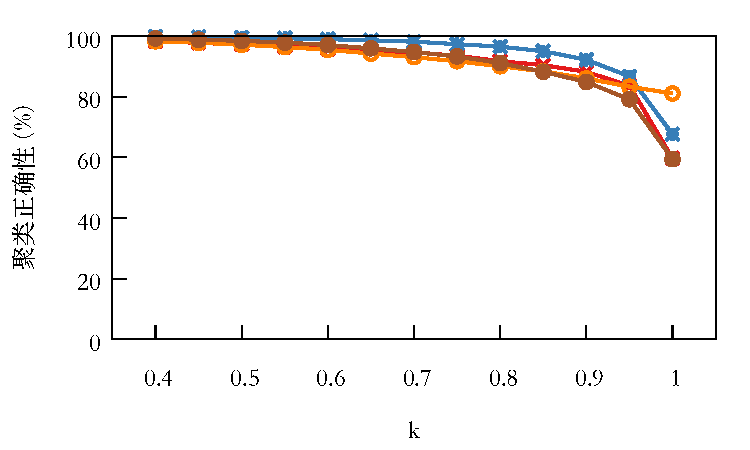
\includegraphics[width=\linewidth]{clu-impact-d-fsl-cro.pdf}\\
    \end{tabular}
    \caption{实验4(参数的影响):FSL数据集中参数$k$对基于聚类的攻击的影响(聚类接近度越小越好;聚类正确性越大越好)。}
    \label{fig:cluster-impact-d-fsl}
\end{figure}

图\ref{fig:cluster-impact-d-fsl}给出了针对FSL数据集的实验结果,其中考虑了四个FSL用户的数据(User004,User007,User015和User028)以节省评估时间。 聚类接近度首先随$k$的增加而增加,这是因为聚类的数量(即$\widetilde{m}$)减少并接近$m$。当$k$进一步增加时,聚类数量会从$m$开始下降,并导致聚类间接近度的增加。此外,实验观察到聚类正确性随$k$的增大逐渐减小,这是因为一些非相似的数据段(即,它们的最小块散列不同)被聚合到同一聚类中。这两个结果都表明攻击者可以通过配置一个合适的$k$来平衡聚类的接近程度和正确性的关系。 例如,当我们为User015设置$k = 0.65$时,相应的聚类接近度和正确性分别为1.0\%和94.2\%。这意味着聚类方案的结果高度接近实际分类的结果。
            
\textbf{结论(7):}通过为聚类方法配置适当的参数$k$,攻击可以在未知数据段的最小数据块哈希的前提下得到近似的分类效果。

\begin{figure}[!htbp]
    \centering
    \begin{tabular}{p{.48\linewidth}p{.48\linewidth}}
        \multicolumn{2}{c}{
\includegraphics[width=.7\textwidth]{clu-vm-bar.pdf}}  \\
        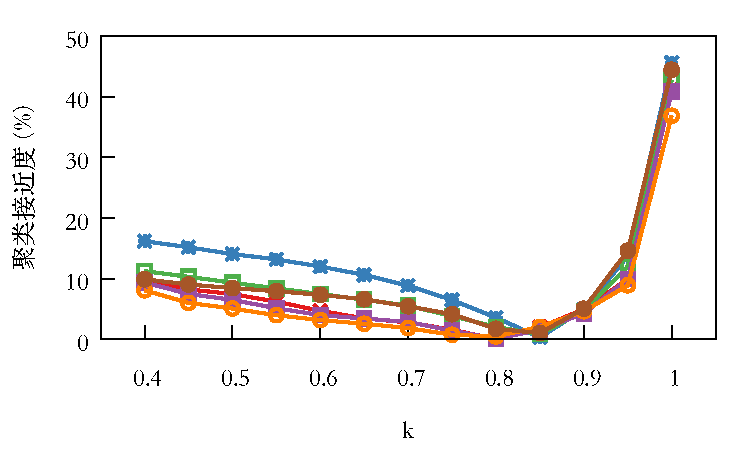
\includegraphics[width=\linewidth]{clu-impact-d-vm-clo.pdf} &
        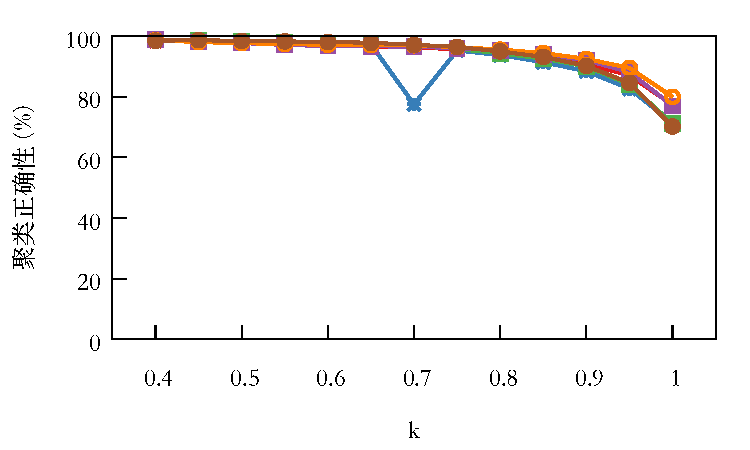
\includegraphics[width=\linewidth]{clu-impact-d-vm-cro.pdf}\\
    \end{tabular}
    \caption{实验4(参数的影响):VM数据集中参数$k$对基于聚类的攻击的影响(聚类接近度越小越好;聚类正确性越大越好)。}
    \label{fig:cluster-impact-d-vm}
\end{figure}

图\ref{fig:cluster-impact-d-vm}给出了针对VM数据集的实验结果。实验观察到所有VM数据集中的用户数据的聚类接近度和正确性与FSL数据集中的用户数据具有相似的趋势。当配置参数$k = 0.8$时,所有VM数据集中的用户数据的平均聚类接近度为3.0\%,相应的聚类正确性高达93.1\%。

\subsection{实验5(攻击效果)} 
\label{sec:exp5}
本实验研究基于聚类的攻击的有效性。由于固定大小的数据段的边界移位问题,它对FSL数据集的有效性很低(在本实验的测试中大约仅有1\%的推理率)。因此,本实验使用VM数据集来评估其有效性。在基于聚类的攻击中,为聚类方法设置参数$ k  = 0.8$,并配置$(u, r, t) = (5000, 100, 0.5)$用于将密文聚类与相应的明文聚类相关联。

在本实验的基准测试中,实验发现基于聚类的攻击中的数据块级推理仅正确地推理出数千个数据块(推理率过低,小于0.01\%)。因此,本文重点研究数据段级的推理,它给出了基于聚类的攻击的有效性的下限。为了与数据块级推理效果的测量保持一致,实验基于每个正确推理的数据段中的唯一性的数据块个数来计算推理率和推理精度。 

\begin{figure}[!htbp]
    \centering
    \begin{tabular}{p{.48\linewidth}p{.48\linewidth}}
        \multicolumn{2}{c}{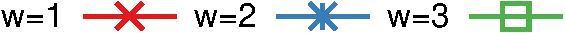
\includegraphics[width=.35\textwidth]{clu-effect-bar.pdf}}  \\
        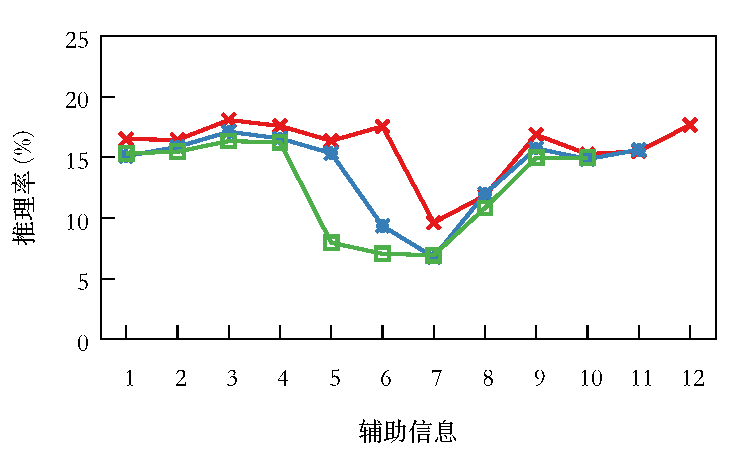
\includegraphics[width=\linewidth]{clu-effect-rate.pdf} &
        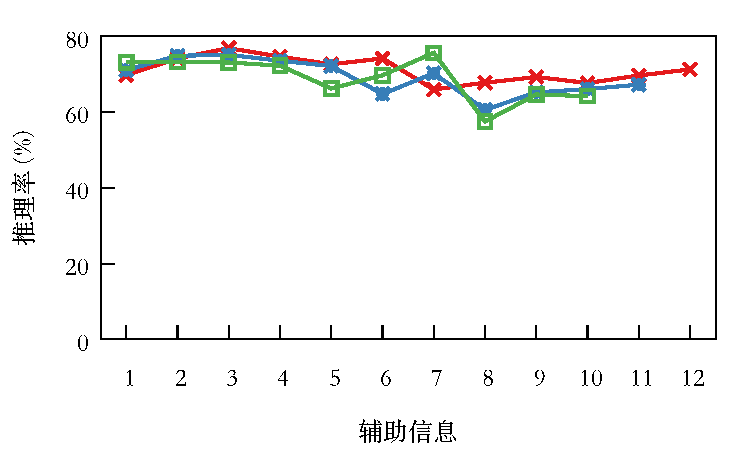
\includegraphics[width=\linewidth]{clu-effect-pre.pdf}\\
    \end{tabular}
    \caption{实验5(攻击有效性):VM数据集中基于聚类的攻击的有效性。}
    \label{fig:cluster-effect}
\end{figure}

本实验采取与实验3(参见\ref{sec:exp3})相同的评估方法,实验结果如图\ref{fig:cluster-effect}所示。具体来说,X轴描述了VM备份数据集中的第$i$(其中1 $ \leq i \leq $ 12)个备份用作攻击的辅助信息,而y轴表示该辅助信息对VM数据集中第$(i + w)$(其中$w = 1,2,3$)个备份的平均推理效果。实验观察到推理率和推理精度都有显著波动。例如,当使用第3个备份作为辅助信息时,攻击的推理率为18.1\%,推理精度为76.8\%($w = 1$);推理率为17.1\%,推理精度为75.0\%($w = 2$);推理率为16.3\%,推理精度为73.0\%($w = 3$)。但当使用第7个备份作为辅助信息时,相应的推理率和推理精度分别下降到9.6\%和65.9\%;6.8\%和71.2\%;以及6.9\%和75.6\%。原因是VM数据集中的备份在第7周之后有大量更新,显著减少了相邻备份间的相关性。平均而言,对于$w = 1,2,3$时,基于聚类的攻击推理出15.8\%,14.0\%和12.6\%密文数据块-明文数据块对,对应的推理精度为71.1\%,69.1\%,和68.9\%。

\section{攻击对安全影响的结果}
\label{sec:case}

到目前为止,本文通过量化正确推理的密文数据块-明文数据块对来检查推理攻击的有效性。然而,这些结果所带来的安全隐患以及频率分析攻击如何带来实际损害仍然是一个悬而未决的问题。在下面的实验中,本文根据原始推理率评估攻击的安全隐患,原始推理率定义为受正确推理的数据块影响的原始数据块的百分比。

\subsection{实验6(安全隐患分析)}
\label{sec:exp6}
实验首先考虑基于分布的攻击,并针对不同类型的文件评估其原始推理率。这一部分使用FSL数据集来进行评估,因为只有FSL数据集包含数据块所属的文件的文件元数据(包含文件的扩展名)。具体来说,本实验关注具有特定扩展名的五种类型的文件(参见表\ref{tab:exp-fsl-file-dis}):office文件,图片文件,程序源代码文件,数据库文件和磁盘映像文件。这些文件占FSL数据集原始内容的60\%以上。

\begin{table}[!htbp]
\small
\caption{实验6(安全隐患分析):基于分布的攻击}
\label{tab:exp-fsl-file-dis}
\centering
\begin{tabular}{|c|c|c|c|c|c|}
\hline

    \multirow{2}{*}{\bf 文件类型} & \multirow{2}{*}{\bf 扩展名} & \multirow{2}{*}{\bf \centering 文件大小范围}  & \multicolumn{2}{c|}{\bf 原始推理率} \\ \cline{4-5} 
    & & &  $\sf Distribution$-$\sf o$ & $\sf Distribution^S$-$\sf o$ \\ \hline
    Office文件 & doc(x), ppt(x), xls(x) & 10KB-1MB   & 4.9\% & 5.3\%\\
\hline
    图片文件 & jpg, png &10-100KB  & 7.7\% & 6.7\% \\
\hline
    程序源代码 & c, h, cpp, java, py & 10-20KB   & 17.1\% & 15.0\%\\
\hline
    数据库文件 & db, po & 20-700KB   & 2.6\% & 2.4\%\\
\hline
    磁盘映像文件 & vmdk, img & 200MB-1GB  & 15.8\% & 16.7\%\\
\hline
\end{tabular}
\end{table}


这一部分应用实验2(参见\ref{sec:exp2})提出的方法的方法,用$\sf Distribution^S$-$\sf o$和$\sf Distribution$-$\sf o$来评估机遇分布的攻击的原始推理率。表\ref{tab:exp-fsl-file-dis}给出了实验结果。两种攻击实例针对磁盘映像文件都具有较高的原始推理率(例如,$\sf Distribution$-$\sf o$为15.8\%,$\sf Distribution^S$-$\sf o$为16.7\%),这因为每个磁盘文件中包含大量很少进行更新的数据块,这些数据块在同一文件中具有很强的数据块局部性。有趣的是,实验观察到程序源代码文件中,尽管每个文件都很小,但基于分布的攻击也具有很高的原始推理率(例如,$\sf Distribution$-$\sf o$为17.1\%,$\sf Distribution^S$-$\sf o$为15.0\%)。其原因是程序源代码文件通常一起存储在文件系统中(例如,属于同一项目的源文件位于相同的目录中)并形成大范围的相关数据块,在文件之间具有很强的数据块局部性。对于小型或分散的文件(例如,Office文件,图片文件和数据库文件),基于分布的攻击的原始推理率相对较低。

\textbf{结论(8):}基于分布的攻击的有效性取决于目标文件的更新频率,文件大小和存储结构。

这一部分使用VM数据集评估基于聚类的攻击带来的安全隐患。具体来说,本实验使用每个VM用户数据的第11个备份来推理该用户相应的第13个中的原始数据内容。由于VM数据集不包含任何元数据,因此本实验根据每个VM快照中的所有数据块计算原始推理率。请注意,本实验在原始推理率的计数中过滤所有全零数据块,因为它们在VM磁盘映像中占有很大比例\citing{jin2009effectiveness},且会对评估的结果产生误导(导致原始推理率结果虚假偏高)。

\begin{table}[!htbp]
\small
    \caption{实验6(安全隐患分析):基于聚类的攻击}
    \centering
    \begin{tabular}{|c|c|c|c|}
    \hline
        {\bf 用户ID} & {\bf 原始推理率} & {\bf 用户ID} & {\bf 原始推理率}\\
    \hline
        1 & 13.2\% & 2 & 22.4\% \\ 
    \hline
        3 & 25.7\% & 4 & 28.4\% \\ 
    \hline
        5 & 18.5\% & 6 & 30.8\% \\ 
    \hline
    \end{tabular}
\label{tab:exp-vm-user-cluster}

\end{table}

这一部分使用与实验5(参见\ref{sec:exp5})相同的配置,并在通过数据段级推理来评估原始推理率。 表\ref{tab:exp-vm-user-cluster}给出了不同用户数据的原始推理率结果。实验观察到基于聚类的攻击对VM数据集实现了很高的安全威胁。例如,它可以推理出User6的VM备份中高达30.8\%的原始内容。所有用户的平均原始推理率高达23.2\%。

\textbf{结论(9):}基于聚类的攻击严重威胁到VM磁盘映像的机密性。
\section{本章小结}
本章通过6个实验对基于分布的攻击和基于聚类的攻击的相关参数的影响、攻击的有效性以及两种攻击手段对真实世界数据集的安全威胁进行了验证与分析,提出了9个根据实验观察得出的结论,证明了两种攻击手段的作用和价值。

